\section{Benchmark Construction and Evaluation Protocol}
\label{sec:method}

Isolating genuine material-conversion effects requires separating shader changes from scene sampling variability, path-tracing noise, runtime environment differences, and coordinate readout artifacts. We design an invariant \textsc{USD} conversion and deterministic measurement pipeline to control each source systematically.

\paragraph{Geometry-locked shader conversion (\textsc{ConvertAsset})}
Given a source \textsc{USD} scene authored with NVIDIA \textsc{MDL} material networks (\original), \textsc{ConvertAsset} recursively traverses references, payloads, sublayers, variant sets, and texture bindings, producing a parallel asset tree (\converted) whose shaders are translated into portable \usdps{} graphs. Mesh vertices, collision bounds, object transforms, camera parameters, and light placement remain identical; only surface optics---color response, metallic specularity, glass transmission, and indirect reflections---change because \usdps{} approximates multi-lobe \textsc{MDL} \textsc{BSDF}s with a unified metallic--roughness shader model (\ref{app:appearance} and~\ref{app:materials}). The translation rules depend solely on scene materials and receive no visual model feedback.

\begin{figure*}[!t]
\centering
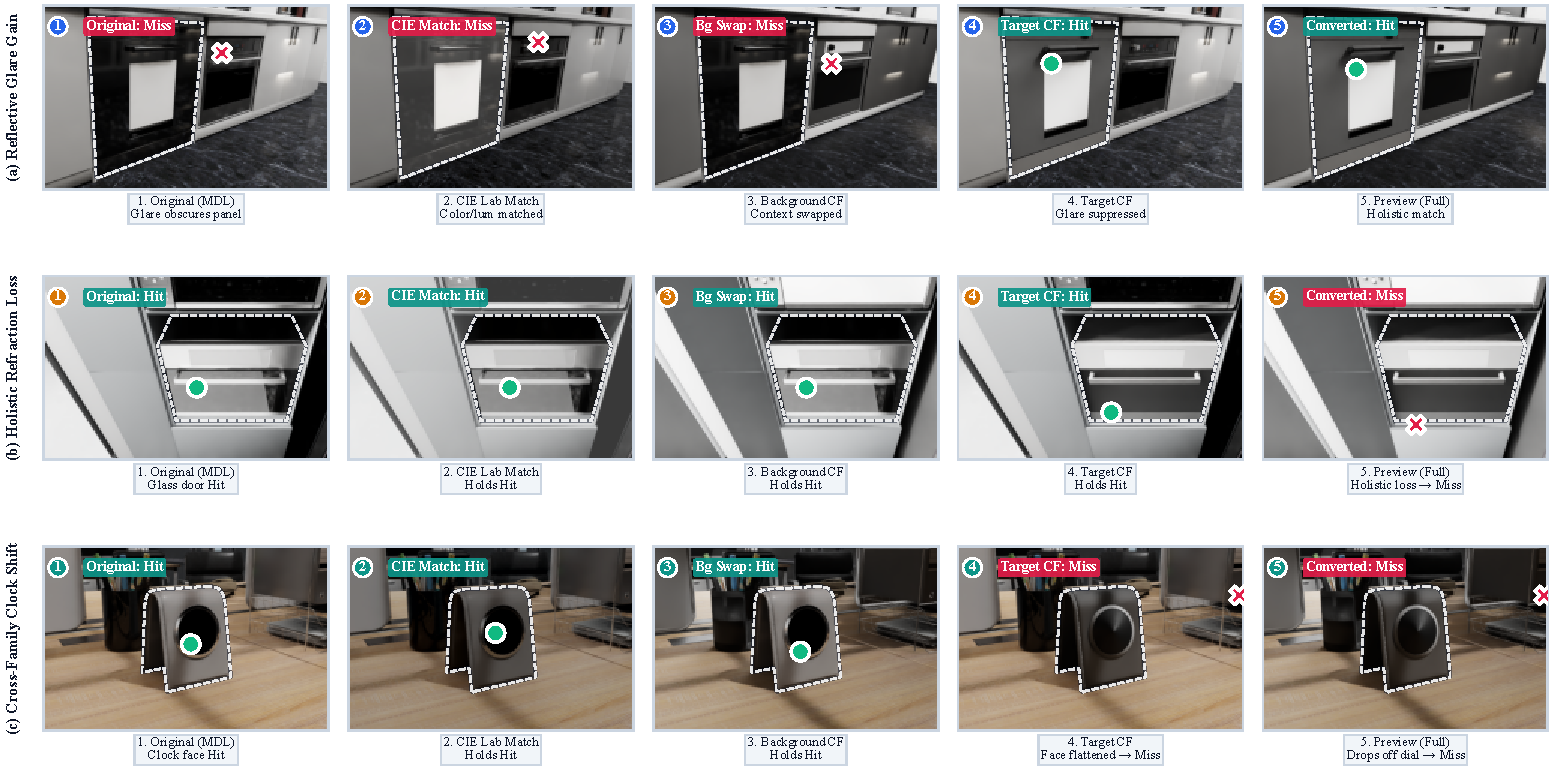
\includegraphics[width=\textwidth]{fig2_case_workflows.pdf}
\caption{\textbf{Representative optical mechanisms and five-condition counterfactual progressions (\textsc{Qwen3-VL-8B} and \textsc{InternVL3.5-8B-HF}).}
Each row traces one target through: (1)~\original\ (\textsc{MDL}) $I^O$, (2)~$\mathrm{CIE}~L^*a^*b^*$ photometric-matched control $I^{\text{photo}}$, (3)~background-only swap $I^B$, (4)~target-only swap $I^T$, and (5)~\converted\ (\texttt{UsdPreviewSurface}) $I^F$.
\emph{(a) Reflective Glare Gain (\textsc{Qwen3-VL-8B}):} glare removal inside the dishwasher silhouette ($I^T, I^F$) flips Miss $\to$ Hit whereas photometric recoloring alone fails ($I^{\text{photo}}$ Miss).
\emph{(b) Holistic Refraction Loss (\textsc{Qwen3-VL-8B}):} $I^O, I^{\text{photo}}, I^B$, and $I^T$ all retain Hit, whereas full scene conversion ($I^F$) flips Hit $\to$ Miss via a $2{\times}2$ scene--target interaction.
\emph{(c) Cross-Family Clock Shift (\textsc{InternVL3.5-8B-HF}):} target dial flattening in $I^T$ and $I^F$ shifts the predicted point off the arched desk clock (Hit $\to$ Miss).}
\label{fig:cases}
\end{figure*}

\paragraph{Thirty-scene benchmark and counterfactual pairs}
Our benchmark comprises \textbf{30 independent SimReady scenes} from \textsc{GRScenes} (20 residential and 10 commercial scenes), partitioned at the scene level prior to any feature fitting into \textbf{15 training (240 pairs), 5 validation (80 pairs), and 10 held-out test scenes (160 pairs)}. In each scene, eight distinct visible object instances are rendered from natural camera viewpoints at $1024 \times 768$ resolution, yielding \textbf{240 objects and 480 paired captures (960 images)}. Every target has a clear referring prompt (\texttt{"Point to the \dots"}) verified across both shader states and a pixel-exact segmentation mask $M_i^v \in \{0,1\}^{768 \times 1024}$ exported directly from the simulator. An automated mask-support check confirms zero empty masks and bit-identical target masks ($\mathrm{IoU} = 1.000$) in \textbf{473/480} pairs; the remaining 7 pairs exhibit subtle thin-rim anti-aliasing or alpha-cutout boundary shifts ($\mathrm{IoU} \ge 0.96$), tested explicitly via a dedicated sensitivity subset (Section~\ref{sec:mechanisms}). Three stratified control scenes (48 pairs, 96 images) provide three independent path-tracing re-renders each under fixed geometry and \original\ materials to quantify rendering variance. Figure~\ref{fig:cases} illustrates the five image conditions ($I^O, I^{\text{photo}}, I^B, I^T, I^F$) across three representative optical cases.

\begin{figure*}[!t]
\centering
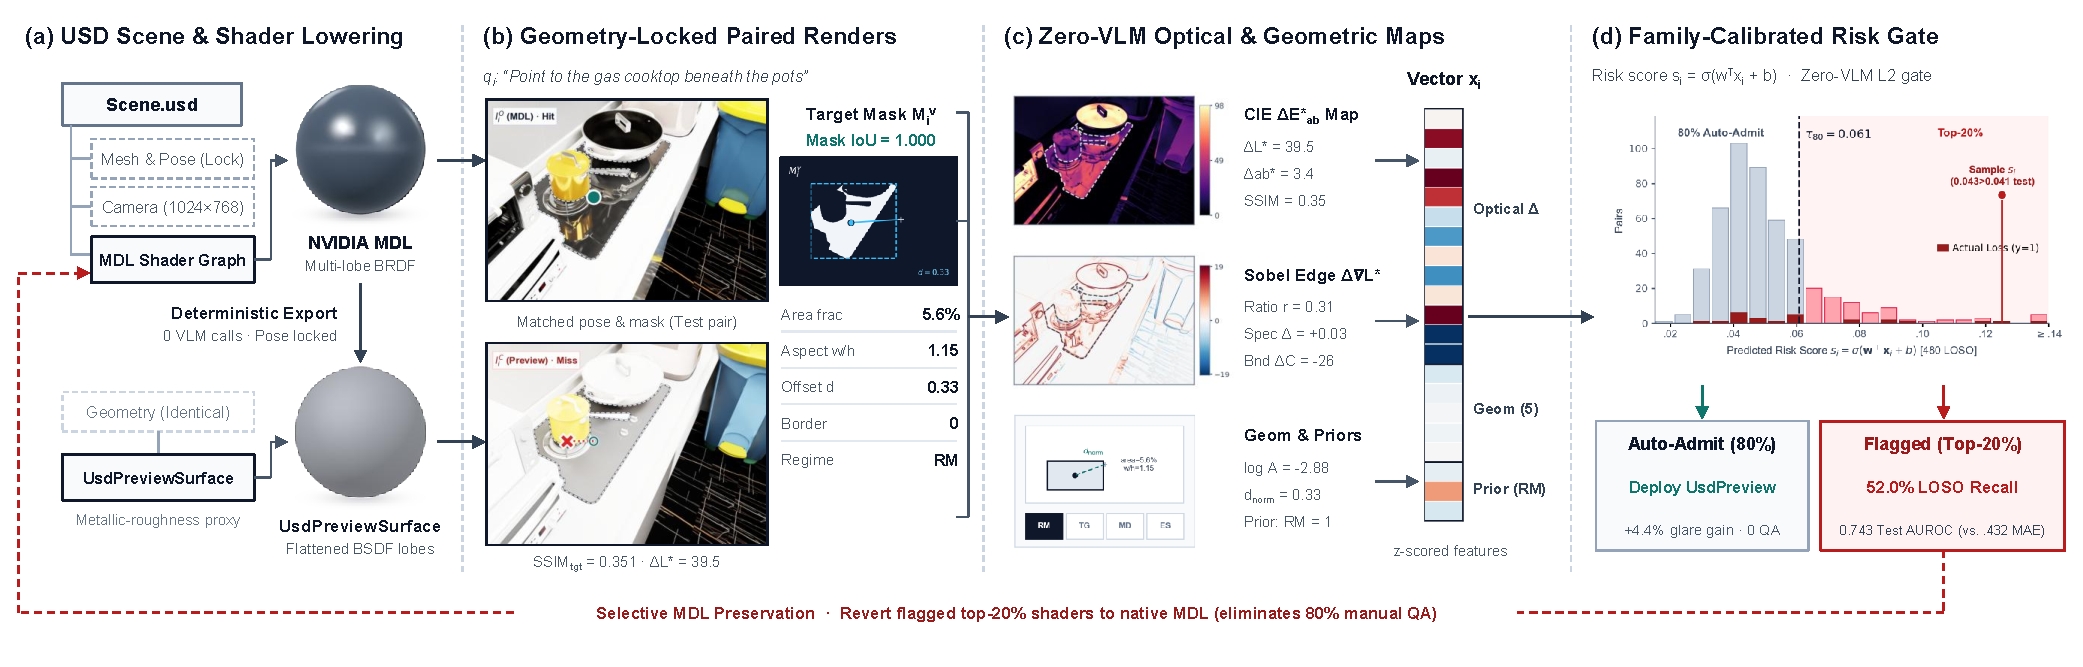
\includegraphics[width=\textwidth]{fig3_pipeline.pdf}
\caption{\textbf{End-to-end \textsc{ConvertAsset} shader-lowering and zero-\textsc{VLM} pre-deployment risk-gating pipeline.}
\emph{(a)} Deterministic \textsc{USD} export lowers multi-lobe \textsc{NVIDIA MDL} shading graphs into \texttt{UsdPreviewSurface} under locked meshes, poses, and camera extrinsics ($0$ \textsc{VLM} calls).
\emph{(b)} Geometry-locked paired renders $(I_i^O, I_i^C)$ and pixel-exact simulator masks $M_i^v$ expose directional localization regressions on held-out targets (here \textsc{Qwen3-VL-32B} flips Hit $\to$ Miss on a flattened reflective cooktop).
\emph{(c)} Zero-\textsc{VLM} perceptual ($\mathrm{CIE}~\Delta E_{ab}^*$), structural (\textsc{SSIM}, \textsc{Sobel} $\Delta\nabla L^*$), mask-geometry, and coarse regime-prior cues form a standardized feature vector $\mathbf{x}_i$.
\emph{(d)} A family-calibrated $\ell_2$ logistic gate scores regression risk $s_i = \sigma(\mathbf{w}^\top \mathbf{x}_i + b)$, auto-admitting $80\%$ of low-risk assets while routing the highest-risk $20\%$ back to selective \textsc{MDL} preservation ($52.0\%$ \textsc{LOSO} recall; $0.743$ test \textsc{AUROC} vs.\ $0.432$ global \textsc{RGB MAE}).}
\label{fig:pipeline}
\end{figure*}

\paragraph{Readout standardization, parser qualification, and paired estimands}
Because inconsistent coordinate conventions or non-deterministic sampling can masquerade as visual sensitivity (\ref{app:readout}), every evaluation executes unquantized \texttt{torch.bfloat16} inference (\texttt{device\_map="auto"}) with deterministic greedy decoding ($T{=}0$, \texttt{do\_sample=False}) under a uniform CUDA software environment, using a single canonical $0\text{--}1000$ normalized pointing prompt:
\begin{quote}\footnotesize\ttfamily
<query> Use normalized 0-1000 coordinates:\\
(0,0) top left, (1000,1000) bottom right.\\
Return exactly one line: Point: x, y
\end{quote}
To accommodate each family's native coordinate syntax without truncating bounding boxes or distorting predictions, every evaluated checkpoint first passes a 24-input pilot qualification gate ($\ge 90\%$ valid coordinate parses; Section~\ref{sec:grounding}, \ref{app:readout}), selecting one deterministic parser mode per family:
\begin{itemize}
    \item \texttt{strict}: exact \texttt{Point:\ x, y} format in $[0, 1000)$ (\textsc{Qwen3-VL-8B/32B}, \textsc{InternVL3.5-8B-HF}; $100\%$ pilot valid).
    \item \texttt{flex\_1000}: accepts \textsc{Qwen3-VL-2B}'s bare \texttt{(x, y)} tuples, JSON \texttt{point\_2d}, and 4-number box midpoints ($91.7\%$ pilot valid; $96.5\%$ full-benchmark valid).
    \item \texttt{molmo2\_1000}: extracts \textsc{Molmo2-8B}'s native \texttt{<points coords="1 1 x y">} and \texttt{<Point:\ x y>} tags ($100\%$ pilot valid; $99.1\%$ full valid).
    \item \texttt{unit\_float\_xy}: rescales \textsc{LLaVA-NeXT-Mistral-7B}'s unit-normalized $[0, 1]$ boxes and points to $0\text{--}1000$ midpoints ($100\%$ pilot valid; $99.2\%$ full valid).
\end{itemize}
For pair $i$ under condition $v \in \{O, C\}$, parsed coordinate $(u_i^v, v_i^v)$ maps to pixel $(u_i^v W / 1000,\, v_i^v H / 1000)$, defining binary grounding success $H_i^v = \mathbf{1}[(x_i^v, y_i^v) \in M_i^v]$. Beyond marginal hit rates $H^O$, $H^C$, and net delta $\Delta H = \mathbb{E}[H_i^C - H_i^O]$, we track paired decision-turnover rates:
\begin{align}
\mathrm{Loss} &= \Pr(H_i^O{=}1,\, H_i^C{=}0), \quad
\mathrm{Gain} = \Pr(H_i^O{=}0,\, H_i^C{=}1), \notag\\
\mathrm{Flip} &= \mathrm{Loss} + \mathrm{Gain},
\label{eq:turnover}
\end{align}
alongside conditional regression risk $\Pr(H_i^C{=}0 \mid H_i^O{=}1)$ and valid-pair Euclidean displacement $\Delta p_i = \|p_i^C - p_i^O\|_2$ in pixels. Because 16 camera pairs share each 3D environment, all confidence intervals and paired contrasts use \textbf{10,000-draw scene-cluster bootstrap resampling} over the $S=30$ scenes. Figure~\ref{fig:pipeline} illustrates the combined shader-lowering and zero-\textsc{VLM} risk-gating architecture.

\paragraph{Closed-loop navigation protocol (\textbf{RQ4})}
Section~\ref{sec:navigation} examines \textsc{InternNav/DualVLN} \citep{Wei2026Ground} over 99 paired unseen episodes across three KuJiaLe \texttt{val\_unseen} apartments (33 episodes per scene, 198 rollouts) sharing identical language instructions, starting poses, and step budgets.
